% !TeX root = ../main.tex
\chapter{State of the Art and Literature Review}
\label{ch:state-of-art}

\section{Fundamentals of Industrial Robotics}
\label{sec:fundamentals-industrial-robotics}
Industrial robots are a central part of modern manufacturing because they combine repeatability, precision, and the ability to perform physically demanding operations over long production cycles. The international standard ISO 8373 describes an industrial robot as a reprogrammable and multipurpose manipulator with three or more programmable axes \cite{ISO8373}. In practice, such systems are used for handling, assembly, welding, forming, and many other operations in which stable and repeatable motion is required.

A typical industrial robot consists of several actuated joints that provide the degrees of freedom (\acs{dof}) needed to position and orient an end-effector in three-dimensional space. The task-relevant reference point is usually defined by the \ac{tcp}, which links the robot motion to the physical tool or gripper. Forward and inverse kinematics describe the relationship between joint variables and the Cartesian pose of this reference point, forming the basis for motion planning and robot control \cite{craig2005robotics}.

Robot programming can be understood as a spectrum of abstraction levels. At the lower end, the operator or programmer explicitly defines poses, trajectories, and process sequences. At higher levels, the user specifies the intended task, while the system derives executable actions and motion commands. Industrial practice still relies heavily on manual and offline programming, but research has increasingly moved toward higher levels of abstraction, including task-level programming and skill-based approaches that reduce the need for detailed low-level motion specification \cite{Pan2012Survey,Kruger2019}.

This shift is especially important for manufacturing tasks that are not simple repetitions of a fixed motion. In applications such as robotic sheet metal bending, the robot must handle changing workpiece geometry, limited workspace, tool access constraints, and possible reorientation steps. These characteristics make the task more demanding than conventional pick-and-place operations and motivate the need for a broader review of robot programming methods, press brake automation, and integrated planning approaches.

\section{Sheet Metal Bending and Press Brake Systems}
\label{sec:sheet-metal-bending-press-brake-systems}
Sheet metal bending is a forming process in which a flat metal sheet is plastically deformed along one or more bend lines. In a press brake, the sheet is positioned between a punch and a die, and the bending result depends on tool geometry, material properties, sheet thickness, bend sequence, and applied force \cite{Pahl2007EngineeringDesign}. The process is common in industrial production because it can create a wide range of functional parts from relatively simple sheet blanks.

Figure~\ref{fig:press_brake_system} illustrates a typical robotic press brake setup, where an industrial robot is integrated with the bending machine to automate handling operations.

\begin{figure}[htbp]
\centering
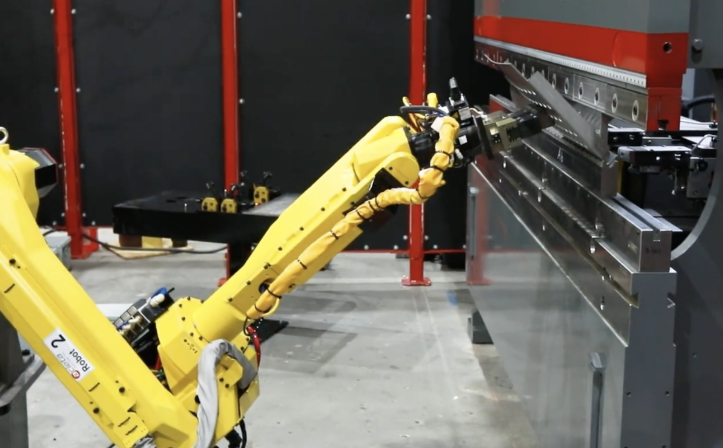
\includegraphics[width=0.85\textwidth]{figures/press_brake_system.png}
\caption{Robotic press brake bending system with integrated robot handling (Source: \cite{acieta_press_brake}).}
\label{fig:press_brake_system}
\end{figure}

In automated press brake cells, the robot usually picks the flat sheet, positions it at the tooling, supports it during bending, reorients it between process steps, and unloads the final component. This automation can improve repeatability and reduce direct operator involvement, particularly in repetitive production settings \cite{Aomura2002RoboticBending}. However, the process is difficult to automate fully because each bend changes the physical shape of the part.

\subsection{Process Characteristics and Automation Challenges}
\label{subsec:process-characteristics-challenges}
The changing geometry of the workpiece is one of the defining characteristics of sheet metal bending. A motion that is feasible before one bend may become infeasible after the sheet has been formed, because the part envelope, tool accessibility, and collision conditions have changed. Process planning must therefore consider the bend sequence, the accessibility of the tooling, and the handling strategy together rather than as isolated decisions \cite{Gupta1998SheetMetalBending}.

For robotic handling, these process characteristics lead to several practical challenges. The robot must maintain a stable grasp, avoid collisions with the press brake and the partially formed workpiece, remain inside its reachable workspace, and preserve a suitable orientation for the next operation. In many cases, a single grasp is not sufficient for the full bending sequence, so the workpiece must be placed down and grasped again in a different configuration. These issues are introduced here as process-level constraints; the detailed planning problems of regripping, grasp selection, and trajectory generation are discussed later in Section~\ref{sec:robotic-sheet-metal-bending-system}.

\section{Manual and Teach Pendant Programming}
\label{sec:manual-teach-pendant-programming}
Manual programming with teach pendants is one of the most established methods for programming industrial robots. In this approach, an operator defines the robot motion by jogging the robot to desired positions or by entering Cartesian or joint coordinates. The resulting positions are stored as waypoints and executed in a defined sequence by the robot controller \cite{Siciliano2016Robotics}.

Figure~\ref{fig:teach_pendant} illustrates a typical teach pendant interface used for manual robot programming.

\begin{figure}[htbp]
\centering
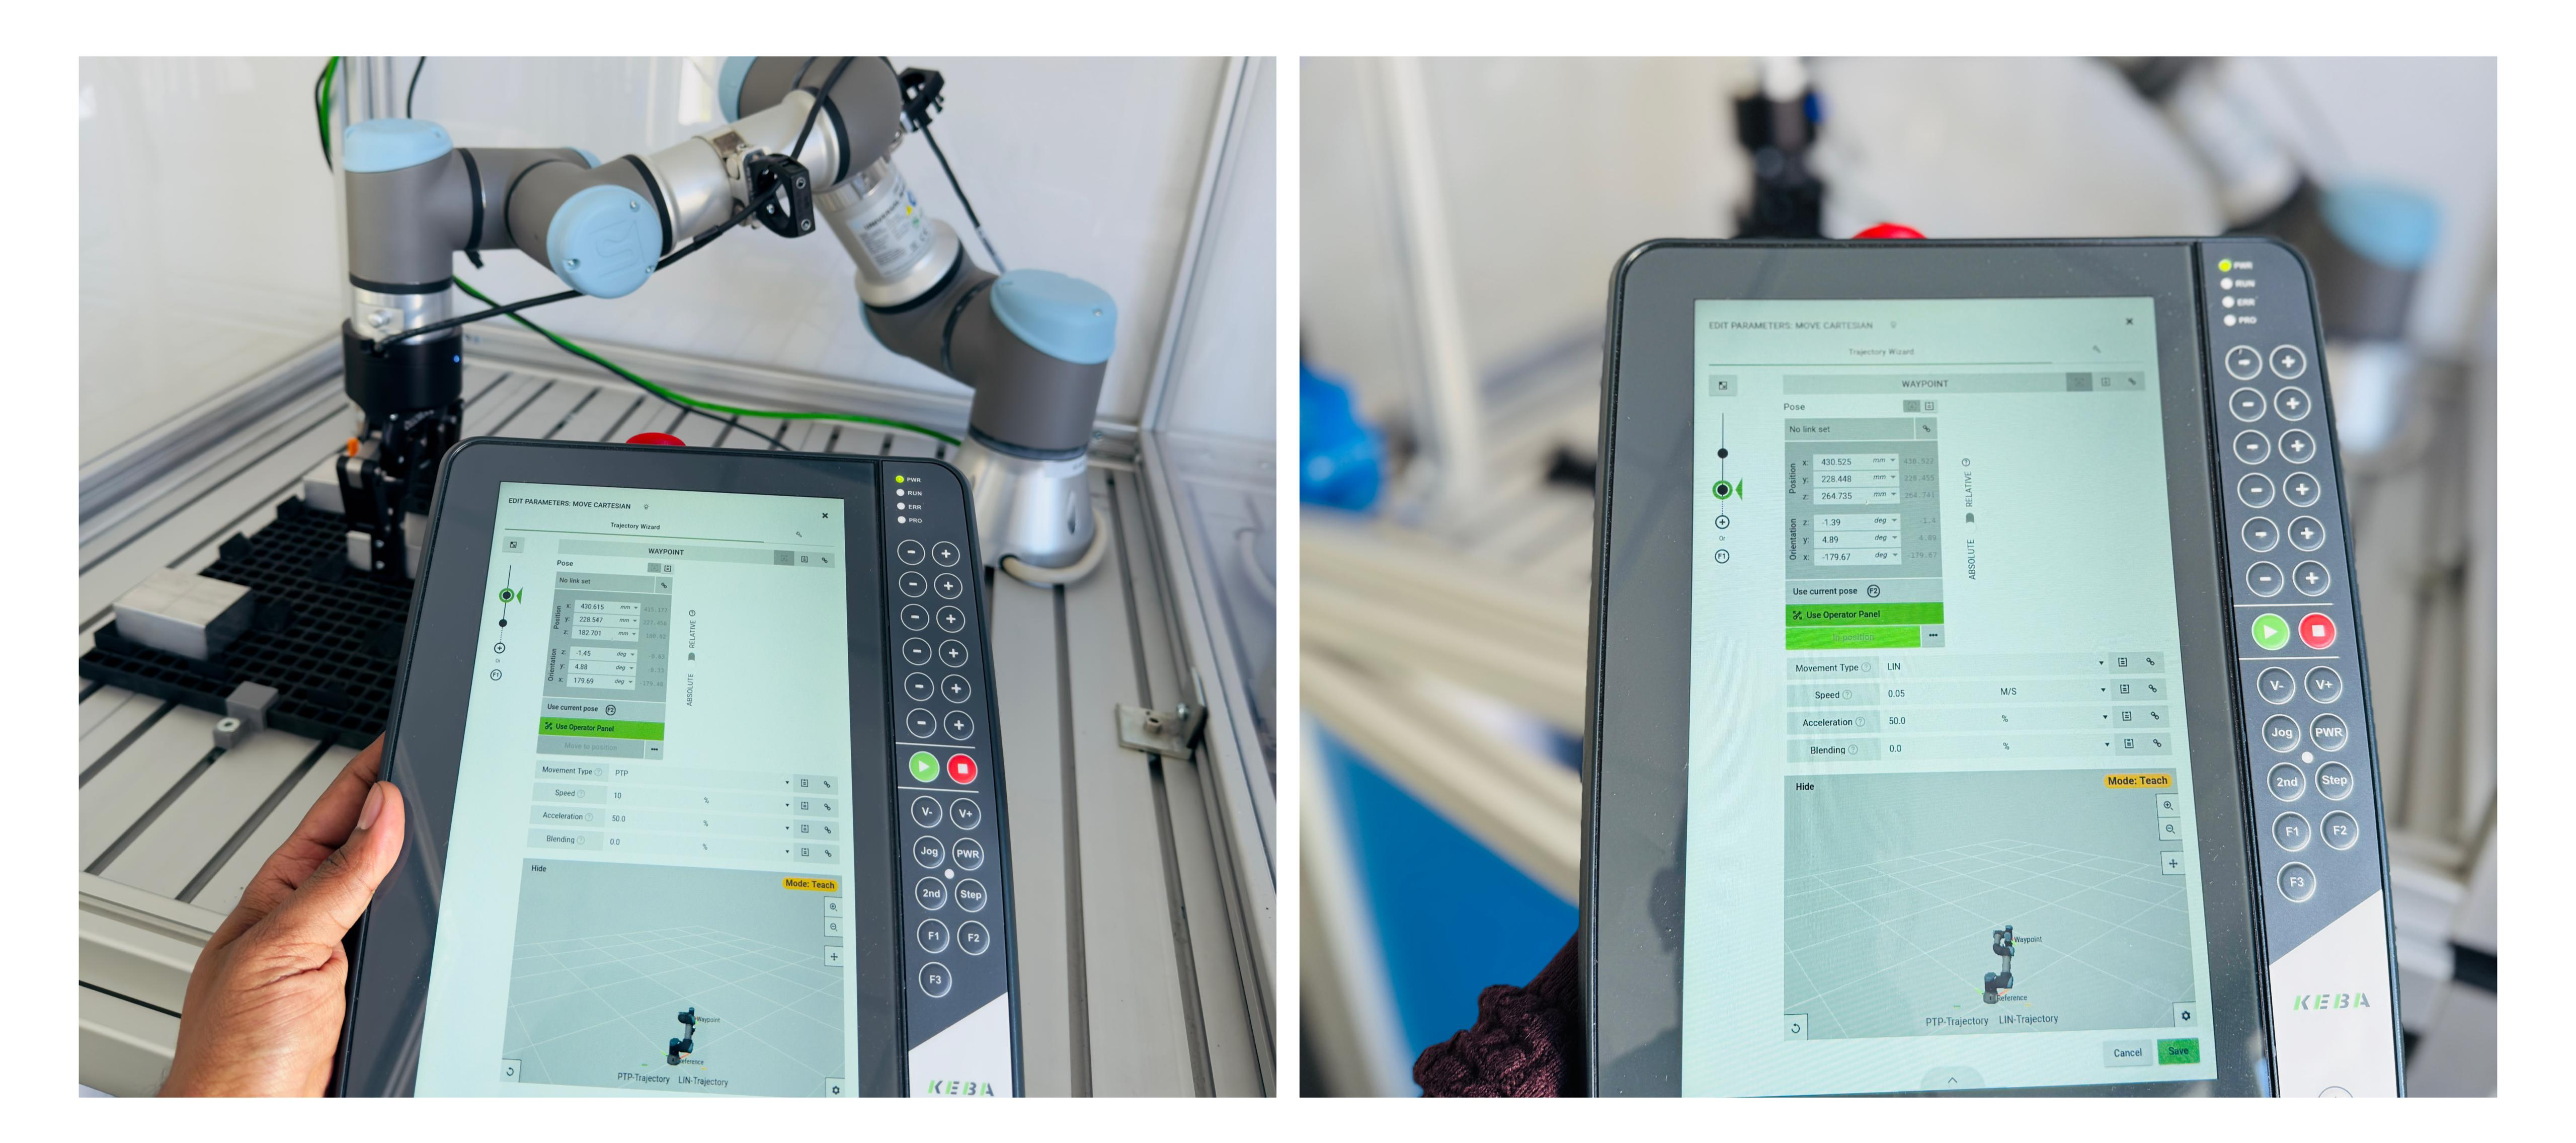
\includegraphics[width=0.75\textwidth]{figures/teach_pendant.png}
\caption{Teach pendant interface for manual robot programming (Source: own work).}
\label{fig:teach_pendant}
\end{figure}
\FloatBarrier

Teach pendant programming remains useful because it gives the operator direct control over the robot and allows immediate verification of individual motions. For stable, repetitive, and well-known tasks, this can be a practical and reliable method. Its limitations become more visible when the process requires many coordinated motions or frequent adaptation to new workpieces.

\subsection{Limitations of Manual Programming}
\label{subsec:limitations-manual-programming}
The main limitation of manual programming is the amount of expert effort required. The operator must understand the robot coordinate system, tool frame, reachability limits, process constraints, and possible collision situations. As the number of waypoints grows, the programming task becomes slower and more dependent on individual experience.

Manual programming is also poorly suited to frequent product changes. If the geometry of the workpiece changes, the robot program often has to be adapted or recreated, even when the process logic remains similar. This makes manual programming inefficient for flexible manufacturing environments with high part variation \cite{Pan2012Survey}. In addition, reachability, collision avoidance, and path quality are not automatically guaranteed; they must be checked and corrected by the programmer.

\subsection{Challenges in Complex Manipulation Tasks}
\label{subsec:challenges-complex-manipulation-tasks}
Robotic sheet metal bending exposes these limitations clearly. The task is not a single transfer motion, but a sequence of handling, positioning, bending, reorientation, and possibly regripping steps. The operator must anticipate how the sheet will change after each bend and must define motions that remain feasible throughout the process.

Regripping is particularly difficult to program manually because it requires coordination between placement, release, new grasp selection, and the next bending operation. Small changes in part dimensions or bend order can alter the required intermediate positions. As a result, manual programming can become time-consuming, difficult to reuse, and vulnerable to inconsistent decisions between operators.

\subsection{Transition Towards Automated Programming}
\label{subsec:transition-towards-automated-programming}
The limitations of manual programming have encouraged the development of methods that raise the level of abstraction. Instead of manually defining every pose, engineers increasingly use virtual commissioning, offline programming, task-level programming, and rule-based planning to reduce direct interaction with the robot. These approaches do not remove all engineering effort, but they shift part of the work from manual waypoint teaching toward model-based planning and validation.

\section{Offline Programming Approaches for Industrial Robots}
\label{sec:offline-programming-approaches}
Offline programming (\acs{olp}) enables robot programs to be prepared and tested in a virtual environment before they are executed on the physical robot. In contrast to teach pendant programming, \acs{olp} decouples programming from production, allowing engineers to develop, simulate, and validate robot tasks without occupying the real workcell \cite{Pan2012Survey}.

Figure~\ref{fig:olp_environment} illustrates an offline programming environment, where a virtual model of the robot, tooling, and workcell is used to simulate and validate motion trajectories.

\begin{figure}[htbp]
\centering
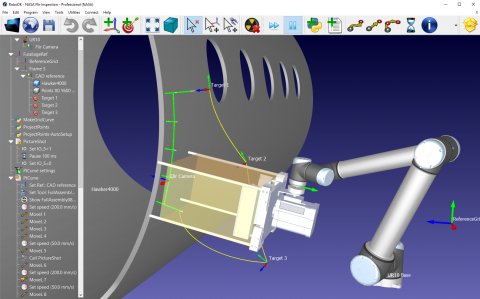
\includegraphics[width=0.85\textwidth]{figures/olp_environment.png}
\caption{Offline robot programming environment with CAD-based simulation (Source: \cite{RoboDK2024}).}
\label{fig:olp_environment}
\end{figure}

\acs{olp} systems commonly use geometric models of the robot, tooling, fixtures, and surrounding equipment. These models allow engineers to evaluate reachability, motion paths, and possible collisions before deployment. In this way, offline programming can reduce floor trial-and-error and support earlier detection of workcell or path problems before production is interrupted \cite{Pan2012Survey,RoboDK2024}.

\subsection{Digital Twin and Simulation-Based Programming}
\label{subsec:digital-twin-simulation-programming}
Digital twin concepts extend simulation-based programming by linking the virtual representation more closely to the physical system. A digital twin can support monitoring, validation, and adjustment by combining model-based simulation with data from the real process. In manufacturing, digital twin approaches have been discussed as an important element of smart production systems because they support analysis, synchronisation, and cyber-physical integration \cite{Tao2019}.

In industrial robotics, tools such as RoboDK, ABB RobotStudio, KUKA.Sim, and drag\&bot provide virtual environments for programming and validation. They support tasks such as visualising the workcell, checking reachability, identifying collisions, and generating executable robot code. These capabilities make simulation-based programming valuable for complex cells where direct trial-and-error programming would be slow or risky.

\subsection{Limitations of Offline Programming}
\label{subsec:limitations-offline-programming}
Despite these advantages, offline programming does not automatically solve the programming problem. The quality of the generated program depends strongly on the accuracy of the virtual model. Differences between the simulated workcell and the real cell can lead to deviations during execution, requiring calibration or manual correction.

Another limitation is that many \acs{olp} tools still require the engineer to define the task sequence, waypoints, and process logic manually. The software can validate and simulate a program, but it does not necessarily decide which grasp to use, when to regrip, or how to generate a complete strategy for a changing workpiece. This limits the usefulness of conventional \acs{olp} for processes such as robotic sheet metal bending, where the task geometry and constraints evolve during execution.

\section{Automatic Robot Program Generation and Rule-Based Approaches}
\label{sec:automatic-robot-program-generation-rule-based}
Automatic robot program generation aims to reduce the need for manual waypoint definition by deriving robot actions from task descriptions, process parameters, geometric input, or formal rules. Instead of programming every motion explicitly, the system computes feasible actions based on the available information and the constraints of the process.

\subsection{Task-Level Programming and Abstraction}
\label{subsec:task-level-programming-abstraction}
Task-level programming is based on the idea that users should describe what the robot should achieve, while the system determines how the task can be executed. Early work on robot programming introduced abstraction layers and symbolic task descriptions as a way to separate task intent from low-level robot motion \cite{LozanoPerez1983}.

More recent approaches use skills, motion primitives, and reusable task modules. A skill may represent an operation such as approaching, grasping, placing, or moving along a constrained path. By combining such skills, complex robot programs can be assembled in a more modular way \cite{Kruger2019}. This improves reusability, but the system still needs reliable mechanisms for selecting valid actions and checking whether the resulting motion is feasible.

\subsection{Rule-Based and Constraint-Based Planning}
\label{subsec:rule-based-constraint-based-planning}
In structured industrial environments, automatic program generation is often implemented through rules and constraints. Rules may describe how a workpiece should be approached, which orientations are allowed, when a regrip is necessary, or which motion types should be used. Constraint-based planning extends this idea by explicitly evaluating geometric, kinematic, and process-related conditions before selecting a solution.

Such methods are attractive because they can produce deterministic behaviour in well-defined applications. However, when product variants and process constraints increase, the engineering effort required to define, adapt, and validate these rules also increases. In robotic sheet metal bending, this issue is especially relevant because bend sequencing, tooling, grasp selection, and robot motion planning are closely coupled \cite{Pan2012Survey,Gupta1998SheetMetalBending}.

For complex manipulation tasks, the main challenge is not only to generate isolated decisions, but to coordinate several planning components. Grasp planning, regrip planning, trajectory generation, reachability checking, and collision avoidance influence each other. If these components are developed separately, a locally valid decision may still lead to an infeasible overall process. Robotic manipulation research therefore emphasizes the importance of integrated planning frameworks, especially when grasping and motion constraints are tightly coupled \cite{bohg2014data}.

\section{Robotic Sheet Metal Bending Systems}
\label{sec:robotic-sheet-metal-bending-system}
Robotic sheet metal bending systems combine an industrial manipulator with a press brake to automate the handling and positioning of sheet metal parts. The robot transfers the sheet, aligns it with the tooling, supports it during bending, and prepares it for subsequent process steps. This integration can improve repeatability and reduce direct manual handling, but it also creates a planning problem that is more complex than ordinary material transfer.

Figure~\ref{fig:robotic_bending_system} illustrates a typical robotic bending setup, where the robot operates in coordination with the press brake to execute a sequence of manipulation and forming operations.

\begin{figure}[htbp]
\centering
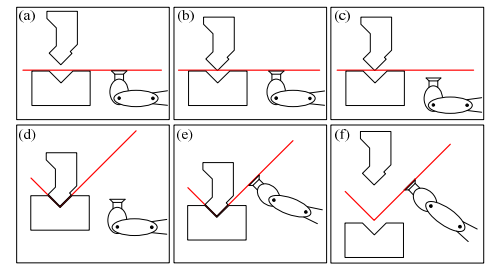
\includegraphics[width=0.75\textwidth]{figures/robotic_bending_system.png}
\caption{Robotic sheet metal bending system with integrated robot and press brake (Source: \cite{Neto2013OLP}).}
\label{fig:robotic_bending_system}
\end{figure}

The process usually starts with a flat sheet, but after every bend the shape of the workpiece changes. This affects collision boundaries, grasp accessibility, tool clearance, and reachable robot configurations. Research on robotic bending has therefore shown that successful automation depends on coordinating process planning with robot motion planning \cite{Gupta1998SheetMetalBending}. The following subsections discuss the main planning aspects that are relevant for this thesis.

\subsection{Regrip Planning in Sheet Metal Bending}
\label{subsec:regrip-planning-sheet-metal-bending}
Regripping is often necessary when the robot cannot execute all bending steps with a single grasp. The required orientation for later bends may conflict with the initial grasp, or the formed geometry may make the original grasp unsuitable. In such cases, the robot places the workpiece at an intermediate location, releases it, and grasps it again in a new configuration.

From a robotics perspective, regrasp planning can be formulated as a search over feasible grasps and transitions between them. A valid sequence must consider grasp stability, reachability, collision avoidance, and the availability of intermediate placements \cite{wan2017regrasp}. In industrial bending cells, however, regripping is often handled through predefined sequences or manually designed rules. This can be reliable for known parts, but it reduces flexibility when the workpiece geometry or bend order changes.

\subsection{Challenges of Regrip Integration in Industrial Systems}
\label{subsec:challenges-regrip-integration-industrial-systems}
The difficulty of regripping is not limited to selecting a new grasp. A regrip decision affects the following trajectory, the accessibility of the next bend, and the risk of collision with both the workpiece and the press brake. Therefore, regrip planning cannot be treated independently from motion planning. In robotic press brake process planning, tooling, grasping, and moving are coupled planning tasks, so a valid bending strategy has to be checked across the process sequence rather than at one isolated step \cite{Gupta1998SheetMetalBending}.

In many existing workflows, grasp selection, regrip decisions, and trajectory validation are performed as separate steps. This separation can create practical problems: a grasp may be stable but unreachable, a regrip pose may be geometrically valid but difficult to approach, or a trajectory may become infeasible after the part has been bent. These dependencies show why integrated planning is important for scalable robotic bending.

\subsection{Grasp Planning for Sheet Metal Handling}
\label{subsec:grasp-planning-sheet-metal-handling}
Sheet metal parts are challenging to handle because they are thin, often large relative to their thickness, and may deform or slip if the grasp is poorly chosen. Vacuum grippers are widely used because they can hold flat sheet surfaces without requiring mechanical clamping around the part. Their performance depends on suction cup placement, contact quality, available holding force, and the distribution of loads during motion \cite{VacuumGripperModeling}.

General grasp planning methods consider object geometry, contact conditions, and task constraints when selecting stable grasp configurations \cite{bohg2014data}. In sheet metal bending, the selected grasp must also leave the bend line and tool access region free. A grasp that is suitable for picking the flat sheet may interfere with a later bending operation, especially after the workpiece geometry has changed. As a result, grasp planning must be linked to the process sequence and not only to the initial sheet geometry.

\subsection{Trajectory Planning in Robotic Bending Systems}
\label{subsec:trajectory-planning-robotic-bending-systems}
Trajectory planning in robotic bending must produce motions that are collision-free, reachable, and compatible with the process constraints. The robot operates close to the punch, die, workpiece, and other cell components, leaving limited room for large avoidance motions. At the same time, it must maintain a suitable orientation so that the sheet can be positioned accurately at the tooling.

Classical trajectory generation methods provide useful foundations for creating smooth and continuous robot motions \cite{Biagiotti2008Trajectory}. However, robotic bending introduces additional constraints because the workpiece geometry changes during the process. The planner must account for evolving collision conditions, workspace limits, possible singularities, and the need to coordinate motion with grasp and regrip decisions \cite{Gupta1998SheetMetalBending}.
In many industrial systems, these challenges are handled by conservative motion templates or manually defined waypoints, which improves reliability but limits adaptability.

\subsection{Limitations of Existing Robotic Bending Systems}
\label{subsec:limitations-existing-robotic-bending-systems}
Existing robotic bending systems have demonstrated that press brake automation is technically feasible, but several limitations remain. Many systems rely on predefined handling strategies and carefully engineered programs. This makes them effective for stable production scenarios, but less suitable for flexible environments where part geometry and process requirements change frequently.

A central limitation is the separation of planning tasks. Grasp planning, regrip planning, trajectory generation, and process validation are often treated as separate activities. This can produce fragmented workflows in which a decision that is valid in one module creates problems in another. For example, a selected grasp may be stable but unsuitable for the next trajectory, or a manually defined path may work for one part variant but fail when the geometry changes.

Another limitation is the continued dependence on expert intervention. Even when simulation and offline programming tools are available, engineers commonly define motion sequences, check reachability, adjust waypoints, and validate process logic manually. This increases setup time and makes adaptation to new parts more difficult. These limitations point toward the need for a unified approach that can combine constraint-aware planning, automated trajectory generation, and structured execution.

\section{Industrial Software Platforms and System Implementations}
\label{sec:industrial-software-platforms-system-implementations}
Industrial robot applications are commonly developed with software platforms that support programming, simulation, validation, and execution. These platforms bridge the gap between theoretical planning methods and practical deployment by giving engineers structured tools for building and testing robotic workflows.

\subsection{Simulation and Offline Programming Environments}
\label{subsec:simulation-offline-programming-environments}
Simulation and offline programming environments allow robot programs to be prepared, simulated, and generated before they are executed in the physical cell. They can support reachability checks, collision evaluation, motion visualisation, and the generation of controller-specific robot code, although the exact capability depends on the software platform \cite{Pan2012Survey,RoboDK2024}. These capabilities reduce commissioning risk and make it easier to identify errors before production is interrupted.

Nevertheless, such environments are usually not fully automatic planning systems. They provide powerful tools for validation and development, but the user often remains responsible for defining the task sequence, selecting key poses, and configuring the logic that connects individual operations. For complex manipulation processes, this manual configuration remains a significant part of the engineering effort.

\subsection{Graphical Programming and Integrated Execution Systems}
\label{subsec:graphical-programming-integrated-execution-systems}
Graphical programming platforms such as drag\&bot further reduce the barrier to robot programming by allowing users to assemble workflows from modular function blocks \cite{dragandbot_anyrobot_2025}. Such systems can combine user interaction, robot communication, and runtime execution in one environment. They are useful for implementing and operating robotic applications without requiring extensive low-level programming.

At the same time, graphical execution systems usually depend on workflows and logic that are defined by the user. They can execute and monitor a process, but they do not inherently solve the planning problem of deciding where to grasp, when to regrip, or how to generate a complete trajectory sequence for a changing workpiece. This distinction is important for robotic bending, where the main difficulty lies in coordinating several dependent planning decisions.

\subsection{Relevance to This Thesis}
\label{subsec:relevance-to-this-thesis-software-platforms}
Existing industrial platforms provide a useful foundation for simulation, communication, and execution. Their limitation is not that they lack practical value, but that they still leave much of the task strategy to the engineer. For press brake bending, this means that grasp selection, regrip handling, and trajectory generation often remain manually configured or only partially automated.

The approach developed in this thesis builds on the strengths of such platforms while adding an automated planning layer. The aim is not to replace industrial execution environments, but to reduce the amount of manual task definition required for robotic bending. By generating and validating motion-relevant decisions within a structured pipeline, the system can use existing runtime tools while improving adaptability to changing workpiece conditions.

\section{Research Gap and Motivation}
\label{sec:research-gap-motivation}
The literature shows a clear development from manual robot programming toward simulation-supported and partially automated methods. Manual programming remains reliable for stable tasks, but it does not scale well when workpiece geometry changes frequently. Offline programming improves safety and commissioning efficiency, yet it still depends on user-defined task sequences and accurate virtual models. Automatic programming and rule-based methods reduce manual effort further, but many approaches focus on individual decisions rather than on the complete bending workflow.

In robotic sheet metal bending, this separation is a major obstacle. The workpiece changes shape after each bend, and this affects grasp feasibility, regrip requirements, collision conditions, and reachable trajectories. A planning decision cannot be evaluated properly if it is isolated from the rest of the process. A grasp that is acceptable at one stage may block tool access later; a regrip pose may be geometrically possible but difficult to reach; a trajectory may be smooth in isolation but unsuitable once the formed part is attached to the robot.

The resulting research gap is the lack of a practically deployable workflow that integrates grasp planning, regrip planning, and constraint-aware trajectory generation for robotic press brake bending. Existing methods and tools provide important foundations, but they do not sufficiently address these interdependent planning tasks as one coordinated process under workspace, kinematic, and process constraints.

Addressing this gap is important for flexible automation. A system that can generate valid target poses, evaluate process constraints, and transform these decisions into executable robot motions can reduce engineering effort and improve adaptability. This thesis therefore proposes an integrated and constraint-aware approach in which automated trajectory generation, workspace-aware planning, and deterministic execution are combined within a structured pipeline.

The identified gap and the proposed direction form the basis for the concept development presented in the following chapter.
